
%\section{Calibration and Validation}
%\section{Validation}
\label{sec:validation}

% VALIDATION TODO
%
% show major effort
% table of results
% show hierarchy
% precisely define cases 
%
%

%
% meshed vanes are 24x more expensive
%

The previous chapters briefly outlined the physical phenomenon under
consideration, the mathematical models proposed to simulate it,
and the numerical solution of these models for a variety of system 
configurations and scenarios. Before these simulations can be used 
as a tool to evaluate proposed system designs, it is necessary to
validate that the physical models in use accurately represent
reality. As defined by Moser {\em et al.}\cite{Moser2012Validating},
``validation is the process of determining whether a mathematical model
is a sufficient representation of reality for the purposes for which the
model will be used--that is, for predicting specified QoIs (Quantities
of Interest) to inform a specific decision.'' 

This chapter contains a discussion of the validation of the
computational models against existing experimental data and high
fidelity simulations. This chapter does not exhaustively detail the
validation studies performed in the course of this study. Rather, this
chapter discusses four representative cases and the overall validation
approach pursued. A more detailed set of validation data is provided in 
Appendix~\ref{app-validation}. The limited validation that was performed
for the 2016 field tests in discussed in Chapter~\ref{sec:field}. 

A challenge in this project is the scarcity of experimental data. Only
two or three cases of experimental measurements are available. These
measurements, for reasons detailed in the next section, are not
sufficient to provide confidence in the output of simulations across a
wide variety  of scenarios. Therefore, a high fidelity model using 
meshed vanes with enforced no-slip velocity boundary conditions along
the surface of the turning vanes was developed. These ``gridded'' runs have
been validated against the experimental data, which they match quite
closely. However, as detailed in Chapter~\ref{subsec:vane}, 
explicitly meshing the vanes would be far too 
prohibitively expensive to permit a rapid exploration of a variety of
system configurations. Instead, this high fidelity model is used 
to generate additional reliable data to permit validation of lower
fidelity models, such as the virtual vanes. Likewise, the results of the
unsteady virtual vane simulations can be used as validation data for a
further reduced, steady Navier-Stokes model. This hierarchy of
validation is shown in Figure~\ref{fig:val_hier}, with data sources that
generate more reliable data at the top, and models that are less
reliable, but also less computationally expensive at the bottom. In
terms of expense, the steady virtual vane model generates a solution in
approximately two minutes, versus twelve hours for the unsteady virtual
vane model. The gridded vanes require another factor of ten in
computational time, and many more man-hours hours of work to generate
the mesh (which were generated using gridgen). An example of one of the
gridded meshes complexity is shown in Figure~\ref{fig:gridded_mesh}. 
Therefore, it is unrealistic to perform parameter sweeps or
system configuration investigations with the gridded vanes and these
results are used only for validation studies. Instead, the
steady model is used, with promising results re-evaluated with unsteady
virtual vane models. %and so on up the hierarchy if more confidence is necessary. 

%
% https://www.draw.io/
%
 \begin{figure}[!htb]
   \begin{center}
    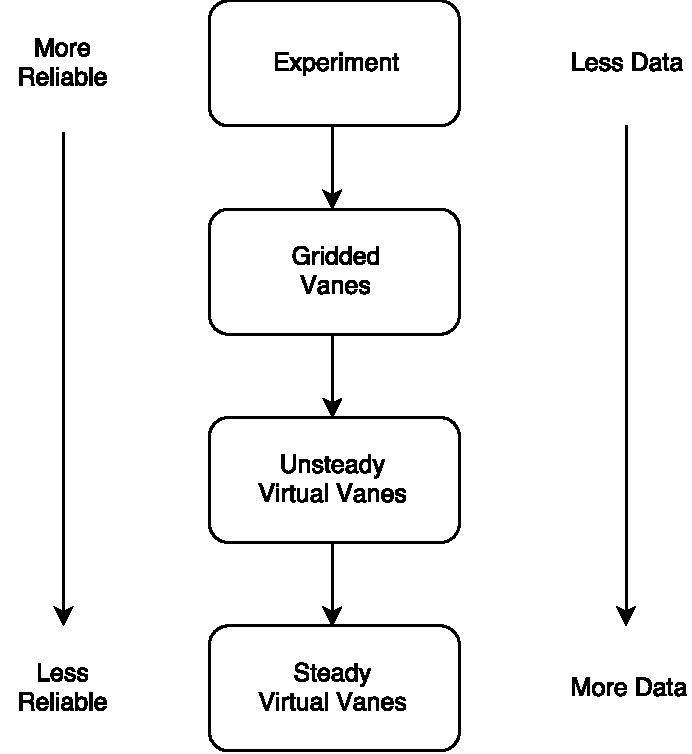
\includegraphics[width = 8 cm]{figs/validation_hierarchy}
    \caption{This figure depicts the validation hierarchy. The
    experimental measurements are at the top, where the data is expected
    to be the most reliable, but simultaneously the most
    limited. Moving down the table leads to simulated data sources that
    are less reliable but increasingly cheaper in time to generate. At
    the bottom are the steady virtual vane solutions.} 
    \label{fig:val_hier}
   \end{center}
 \end{figure}

 \begin{figure}[!htb]
   \begin{center}
    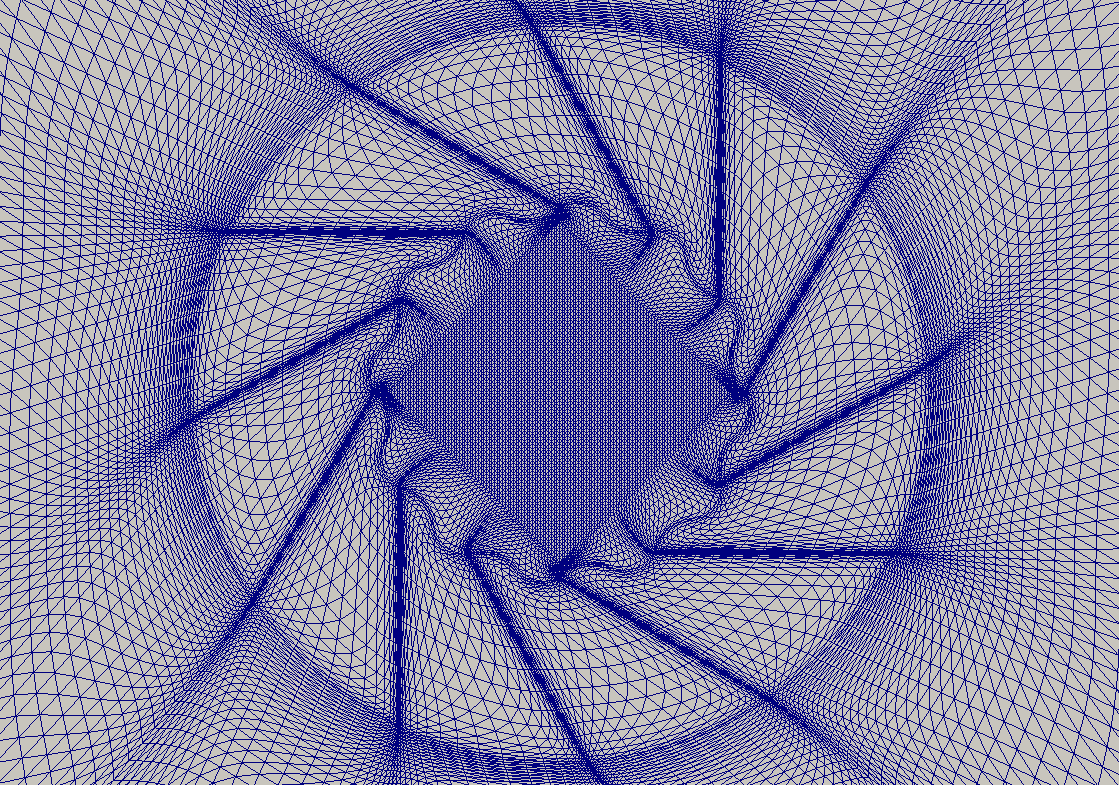
\includegraphics[width = 8 cm]{figs/gridded_mesh_example}
    \caption{An example of the ``gridded'' mesh, where the turning vanes
    are explicitly represented and a no-slip boundary condition is
    imposed on the surface. This mesh was generated using gridgen.} 
    \label{fig:gridded_mesh}
   \end{center}
 \end{figure}

Three kinds of experimental validation data are available. These are
data generated in the laboratory using a heated plate, data from
experiments in the wind tunnel (``Wind-only''), and measurements from field
tests (``Field'') conducted in Arizona. The available data from
these cases and the gridded vanes created to mimic them are are
summarized in Table~\ref{tab:val_data}. Every case shown has been
simulated using the virtual vanes.   

%\large
\begin{table}[h]
\centering
\label{my-label}
\begin{tabular}{l|l|l|l|}
           & Wind-Only                   & Thermal-Only                & Field  \\
  \hline 
Experiment & Straight Vanes $60^{\circ}$ & Straight Vanes $60^{\circ}$ & June 2014   \\
           &                           & Straight Vanes $30^{\circ}$   & August 2014 \\
           &                           & Hybrid (Two tier)             & August 2015 \\
  \hline 
Gridded    & Straight Vanes $60^{\circ}$ & Straight Vanes $60^{\circ}$ & \\
           & Straight Vanes $30^{\circ}$ & Straight Vanes $30^{\circ}$ & \\
  \hline 
\end{tabular}
  \caption{Available truth data from the laboratory experiments 
    (cold wind and thermal-only), the field tests, and the gridded
 vanes.}  
  \label{tab:val_data}
\end{table}
%
%
%
% http://www.tablesgenerator.com/
%
%


%
% experimental challenges
%
%\normalsize
\section{Thermal-Only Validation}
This section provides examples of the validation performed with the
richest data set, the measurements in the laboratory. All of the
thermal-only the data was generated in a laboratory setting at Georgia
Tech. The general system configuration is depicted in Figure
\ref{fig:lab_image}. These data were taken using stereo particle image
velocimetery (PIV) at Georgia Tech by Mark Simpson and Ari Glezer, and
the errors in in measurement and sampling are 
not quoted. The particles are seeded outside of the array vanes and
permitted to naturally convect into the turning vane enclosure. The
particles were from a glycol-water theatrical fog (Rosco Fog Fluid). 
Only velocity measurements are available. Several
potentially important quantities of interest, such as the pressure and
temperature, have not been measured. 

%
% http://convertonlinefree.com/ConvertImageEN.aspx
%
 \begin{figure}[!htb]
   \begin{center}
    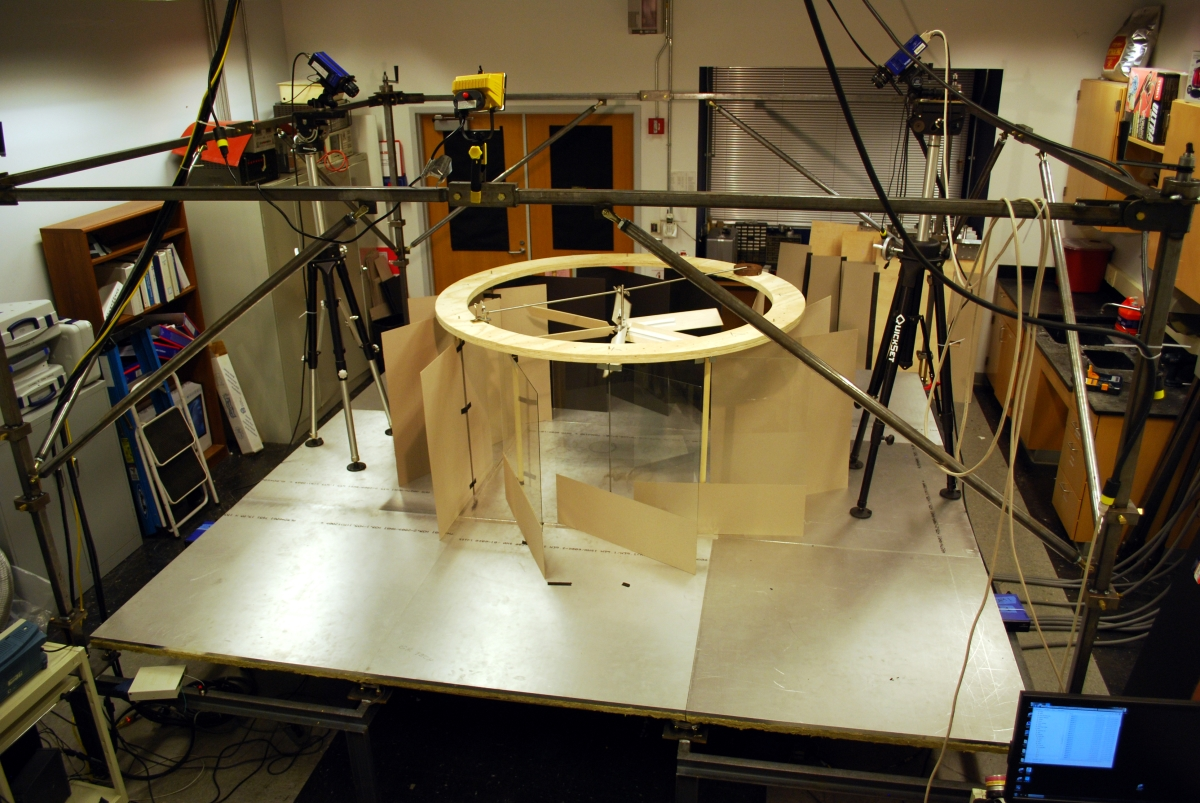
\includegraphics[width = 12 cm]{figs/Optimized-lab_setup}
    \caption{An example of the single tier straight vane laboratory
    configuration. The apparatus is shown with a turbine, but that was
    removed for data gathering. The particles for PIV were seeded
    outside of the turning vanes and entrained into the central region.}
    \label{fig:lab_image}
   \end{center}
 \end{figure}

While no sensitivity analysis has been performed, it is likely that the
largest uncertainty in the laboratory simulation is a result of the
ventilation of the laboratory. The heated plate at the bottom of the
apparatus generates enough heat to cause a significant increase in room
temperature (30+ Kelvin), which greatly impacts the SoV
performance, as the ground to air thermal gradient drives the
vortex. The laboratory is cooled to maintain
temperature by two inlet HVAC ducts into the room. 
%While efforts have been made to characterize the level of ventilation being
%used, these numbers come with non-trivial uncertainties attached. 
One vent continuously provides air at 288 Kelvin with a flow rate estimated 
to be 1 $\text{m}^3$/s.
%(4-6 m/s with an approximate area of 0.2 $m^2$)
The other vent is active only if the room temperature exceeds 301 Kelvin, 
with a flow rate also estimated at 1 $\text{m}^3$/s\cite{mark_comm}.
Finally, the air leaves through the cracks around the laboratory doors and 
exhaust vents. Preliminary results indicated that an inflow rate of 1
$\text{m}^3$/s, the lower bound of the possible inflow rates results in
excessive heating of the room, while inflow conditions at the maximum
inflow rate of 2 $\text{m}^3$/s result in a simulated room that is too cold,
compared to the laboratory.  

Our simulated vortices are sensitive to ambient room temperature and thus 
the inflow rate. It is likely that the laboratory is run where one of
the vents is operating intermittently. 
To mimic these conditions in our simulations, Dirichlet boundary conditions 
on parts of the sides of the computational domain are used to
establish a constant inflow of cool air at the rates 
proscribed by our collaborators. Over the remainder of the side walls, 
adiabatic thermal boundary conditions are are used. 

The most signficant boundary condition disparity is that flow leaves the
domain through the top boundary, instead of out of the sides of the
room. Preliminary results suggested that the SoV phenomenon  was not
sensistive to these boundary condition details. The important element is
the  global energy balance in the room. The flow rate into the room is
adjusted to  1.3 $m^3$/s for the validation results discussed here.  

% \begin{figure}[!htb]
%   \begin{center}
%    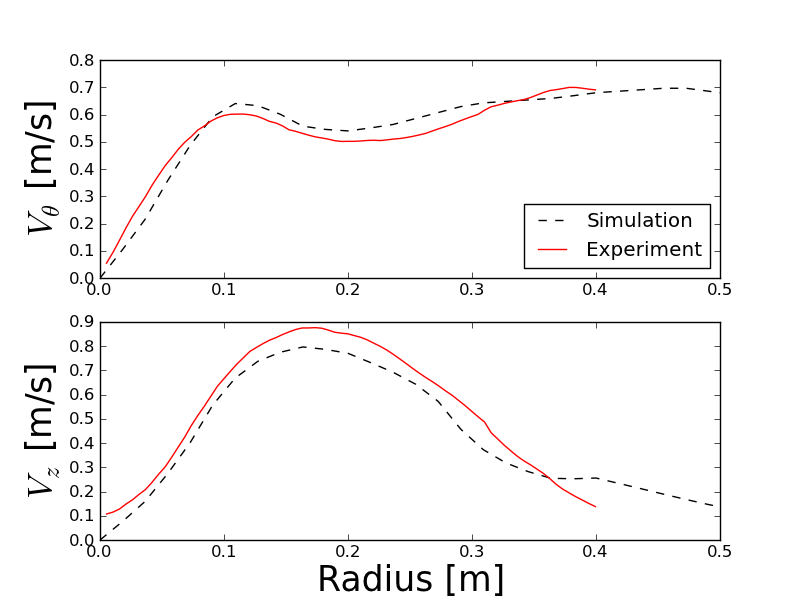
\includegraphics[width = 12 cm]{figs/hybrid_profile}
%    \caption{Azimuthal and vertical velocity profiles as a function of
%    radius. The simulation and experimental data broadly agree, with
%    the simulation also exhibiting the characteristic ``twin-peak''
%    structure of the hybrid vanes in the azimuthal velocity. }
%    \label{fig:lab}
%   \end{center}
% \end{figure}

\begin{figure}[htp!]

  \centering
  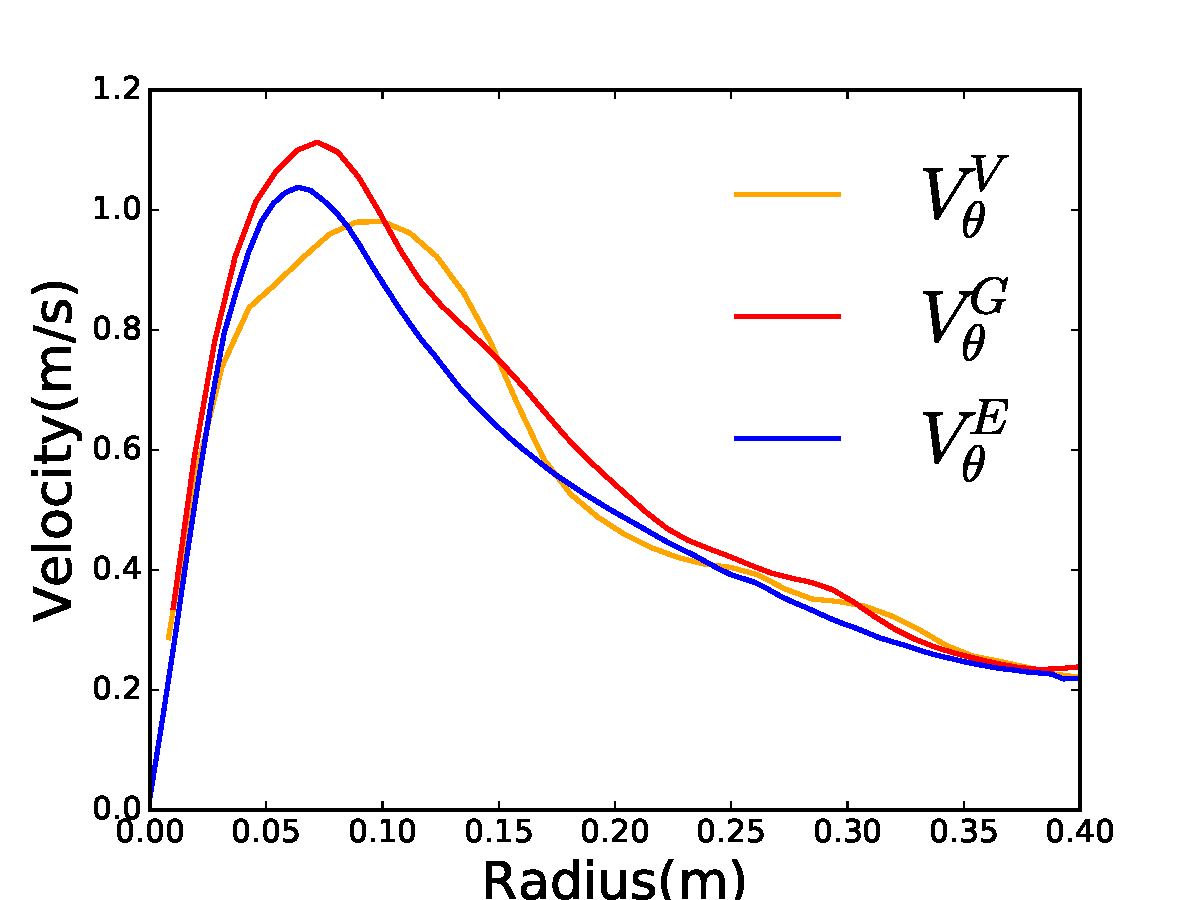
\includegraphics[width =0.47\textwidth]{figs/sim_vs_exp_30_vt}
%  \caption{Azimuthal velocity}
 \hfill
 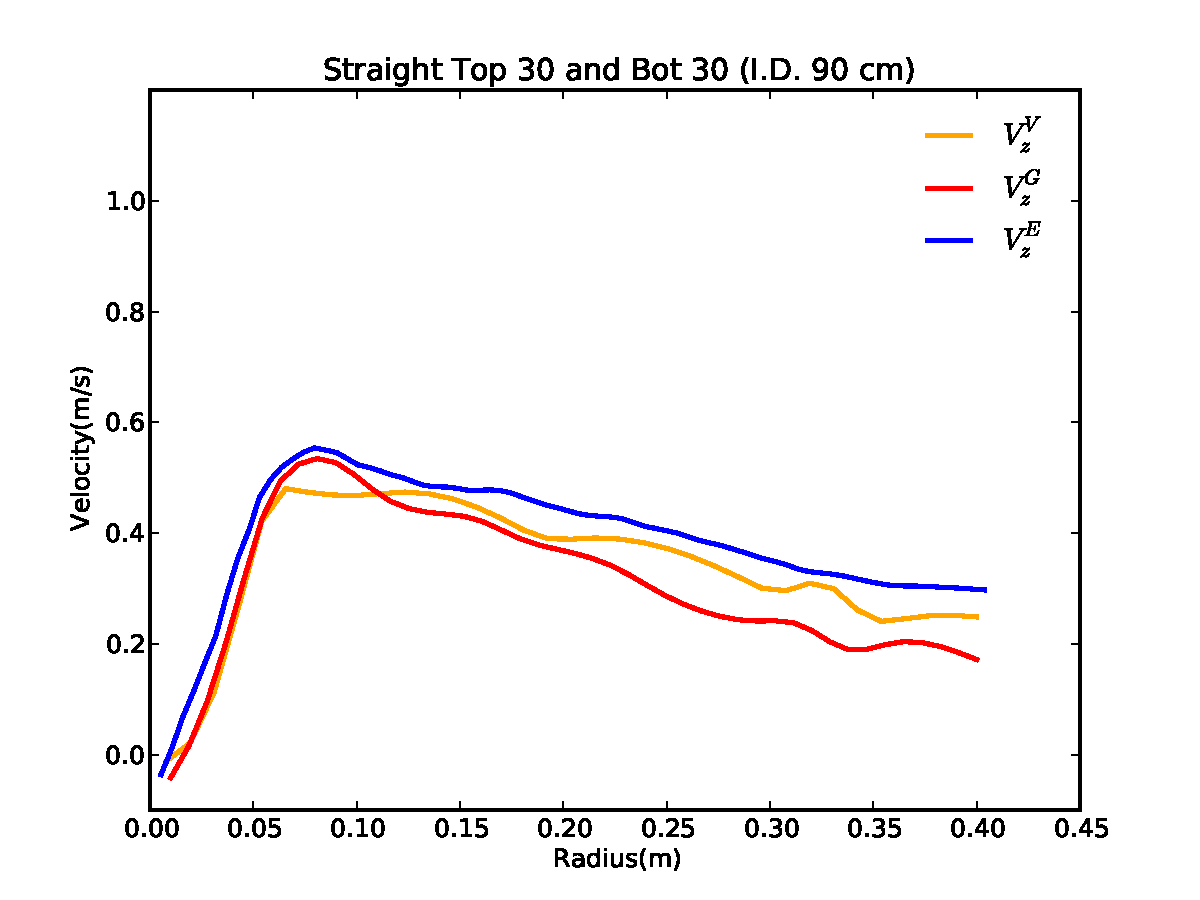
\includegraphics[width =0.47\textwidth]{figs/sim_vs_exp_30_vz}%
 %\caption{Vertical velocity} 
 \caption{Azimuthal (left figure) and vertical (right figure) velocity 
 as a function of radius for the thermal-only cases. Shown are single
 tier straight $30^{\circ}$ vanes. $V_{\theta}^V$ (gold line) is
 the virtual vane simulation, $V_{\theta}^E$ (blue line) the experiment,
 and $V_{\theta}^G$ (red line) the gridded vane. These results were all
 generated by unsteady simulations and then temporally averaged. 
 The lack of smoothness in the data is believed to be
 attributable to finite-time averaging, particularly in the case of the
 gridded vanes, which were expensive calculations. }   
 \label{fig:val_lab}  
\end{figure}

Figure~\ref{fig:val_lab} is a direct comparison
between laboratory measurements for a simple single tier vane
configuration ($30^{\circ}$ straight vanes) and nominally identical
simulations with the gridded and 
virtual vanes. The simulations and experiment broadly agree. The
simulation correctly reproduce the peak structure in the azimuthal
velocity observed for this configuration in the experiment. The gridded
vanes closely represent the peak radial location, while the
virtual vanes over-predict the radial location, likely due to the
increased eddy diffusivity that exists in the virtual vanes. The radial
location and magnitude of peak vertical velocity also closely agrees
with experiment. 

Similar validation comparisons have been made between several other
configurations with similar levels of agreement,  notably the
$60^{\circ}$ single tier straight vane case, and the two-tier hybrid
vanes. Some of these cases are detailed in Appendix~\ref{app-validation}.
These validation studies have provided a level of confidence that our
simulations accurately reproduce the phenomena observed in laboratory.

%\todo{slices and images of thermal only?} 

\section{Wind Cases}

The laboratory thermal vortex experiments described in the previous
section did not include the effects of the wind, but experience in
the field indicated that ambient winds were both pervasive and intense
(see Section\ref{subsec:field_predict} for more details). To ensure that
the virtual vanes accurately represent the impact of ambient winds, a
validation study was performed using the data obtained in the wind
tunnel. 

A numerical experiment was performed in which the 60 degree single tier
straight vanes were placed in a isothermal wind. The boundary conditions
are as detailed in Section~\ref{sec:bc}, but with in iso-thermal
conditions. These results were compared to an identical experimental
configuration placed in a wind tunnel. However, no measurements (of
velocity or any quantity) were made for the vanes in these
conditions. Qualitative comparisons, based on descriptions of observed
structures and videos of smoke visualization were made between the
simulations and the wind tunnel experiments. The initial validation was
found to have significant qualitative differences between the virtual
vanes and the experimental images, with the flow visibly exiting out the
back of the vanes instead of being contained within.  As a result of
this inconsistency, the virtual vane model was refined to include a
separation model, which is detailed in Section~\ref{sec:separation}. The
images  did not identify any inconsistencies between the refined
simulation and experiment.   

%
% Attached in the plate from which we inject the fog from. The holes used
% for seeding are the center one (0.5$B!I(B diameter) and the other 4 ones
% which are 0.25$B!I(B diameter. The smallest holes are for alignment pins in
% the tunnel so disregard those ones. Please note that this file is in
% inches and the previous one in millimeters. 
% Hidalgo Ardana Pablo
%
% 11/26/14
%
However, these results are limited, and are
only for the cold wind, as the wind tunnel did not include a heated plate.
To provide a more quantitative validation study, the virtual vanes were
compared to gridded vanes for a cold wind case. Both cases had identical
boundary conditions, as detailed in Section~\ref{sec:bc}. A two meter
per second inlet velocity was selected. 
Figure~\ref{fig:wind_val} contains images of the simulated averaged
streamwise and  spanwise velocity in a horizontal plane at approximately
the height of the vanes obtained from simulations with gridded and
virtual vanes. 
The streamwise velocity penetrates through the region where the vanes
are aligned with the flow in both the gridded and virtual vanes. This
indicates the virtual vane region as defined in
Section~\label{subsec:vane} is not imposing forcing in locations where
the flow is aligned with the vane direction, as intended. 
The second row contains images of the spanwise velocity, where it can be
seen that the virtual vane case correctly reproduces the direction and
magnitude of velocity inside the vanes. While the wake has similar
structure between the two cases for the streamwise velocity, the
spanwise velocity in the wake is not as closely represented between the
cases. While there are some differences in the
details of these simulations, the overall character of the flow
inside the vanes is quite similar. This demonstrates that the virtual
vane formulation can indeed accurately represent the interaction with the wind.

\begin{figure}
  \centering
  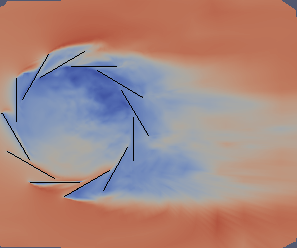
\includegraphics[width=.45\linewidth]{figs/gridded_wind}
  %\caption{Streamwise Velocity: Gridded Vanes}
  \hfill
  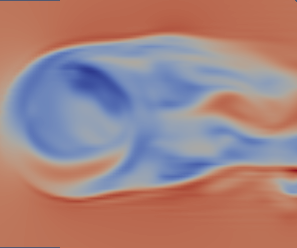
\includegraphics[width=.45\linewidth]{figs/virtual_wind}
  %\caption{Streamwise Velocity: Virtual Vanes}
  \\
  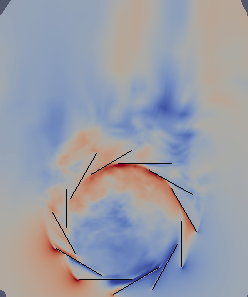
\includegraphics[width=.45\linewidth]{figs/gridded_wind_span}
  %\caption{Spanwise Velocity: Gridded Vanes}
  \hfill
  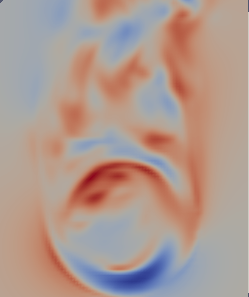
\includegraphics[width=.45\linewidth]{figs/virtual_wind_span}
 %\caption{Spanwise Velocity: Virtual Vanes}
  \label{fig:wind_val}
 \caption{Horizontal slices through the top of the vanes for the
 wind validation cases. On the left are the explicitly gridded vanes,
 and on the right the virtual vanes. The streamwise velocity (top
 images) shows penetration through the region where the vanes are aligned
 with the flow in both the gridded and virtual vanes. The second row
 shows the spanwise velocity, where it can be seen that the virtual vane
 case correctly reproduces the direction and magnitude of velocity
 inside the vanes.} 
\end{figure}


\section{Comparisons between Steady and Unsteady Virtual Vanes}
\label{sec:steady_val}

A the bottom of the validation hierarchy are the steady virtual
vanes. This is expected to be the most inaccurate model. 
Simultaneously, this is by far the cheapest computationally, and 
reduces the run-time from approximately 12 hours (in the case of the
unsteady) to less than two minutes. This much reduced run-time permits
rapid exploration of the SoV configuration space, making the steady
virtual vanes an invaluable design tool. For this reason, the steady
model is used extensively in Chapters~\ref{sec:results} and
\ref{sec:field} to explore new SoV vane design concepts. 

However, the results of the steady cases must first be
compared to the transient case to ensure the output is consistent. 
Figure~\ref{fig:rom_compare} depicts such a case, where the streamwise
velocity in a wind case was used as a direct comparison between the
steady and unsteady virtual vane cases. This was a hot-wind case, with
an ambient freestream velocity of 3 m/s and a temperature gradient of 60
Kelvin. The boundary conditions are precisely as described in
Section~\ref{sec:bc}. 
%The vanes are an axi-symmetric two-tier structure,
%with inner vane angles of  and degrees, respectively. 

These two solutions are similar, with comparable velocity magnitudes and 
consistent signs. A comparison between the azimuthal velocities are
shown in Figure~\ref{fig:rom_az}, which makes clear the more diffuse and
weaker magnitude peak in the steady solution. Ultimately, the steady
solution's principle use as a design tool is driven by the response in
kinetic energy flux to sensitivity to small perturbations in the SoV
design (such as vane or cone geometry). To measure this, a comparison
was made to between steady and unsteady solutions from a base state to
small perturbations in the vane angles. The results of this are shown in
Figure~\ref{fig:rom_it}, where the steady solution typically
underestimates, but broadly agrees with, the change in kinetic energy
flux attributable to a perturbation in the system design parameters. 
It is for this reason that the steady solution is believed to be a
useful tool to explore the system configuration space, as it accurately
represents favorable design adjustments, and so can be used in an
optimization effort to rapidly probe various configurations and drive
the system towards peak kinetic energy flux generation. 

\begin{figure}[htp!]
 \centering
 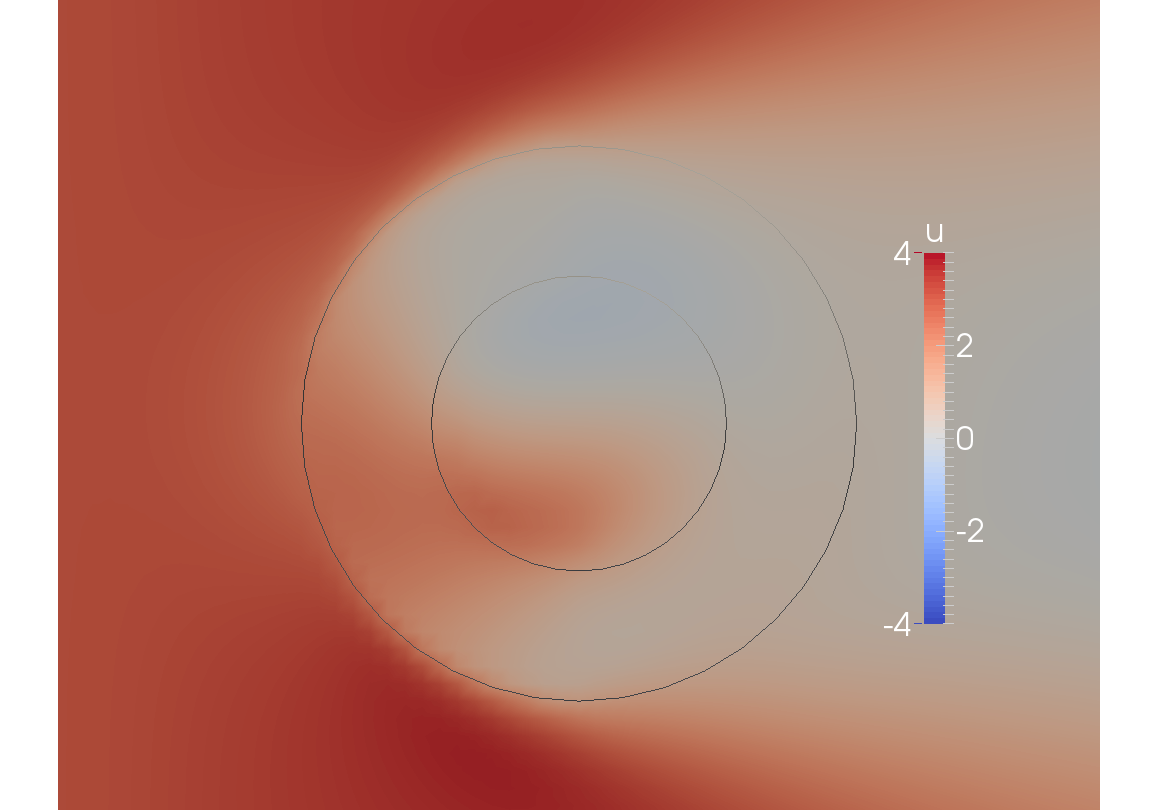
\includegraphics[width =0.47\textwidth]{figs/rom_steady}
 \hfill
 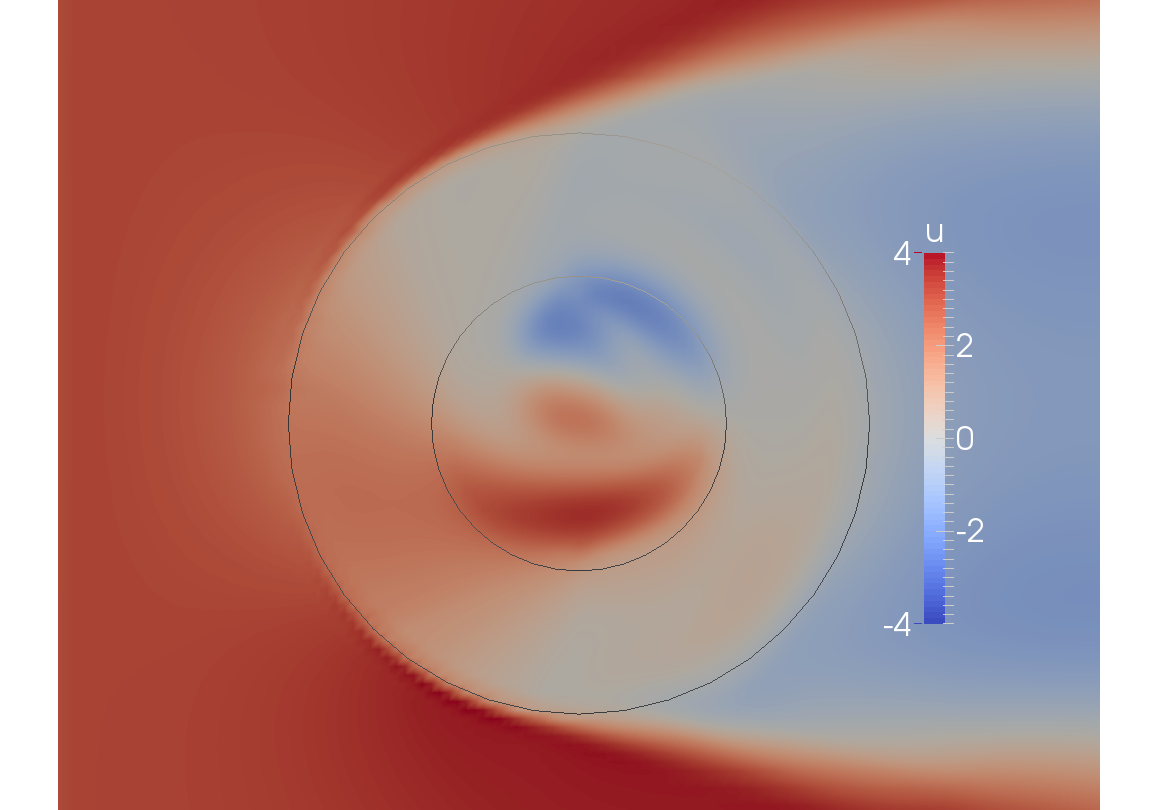
\includegraphics[width =0.47\textwidth]{figs/rom_unsteady}%
 \caption{A comparison between the streamwise velocity in the averaged
 transient virtual vane solution (right image) and the steady virtual
 vane solution (left image). These horizontal slices were taken at the
 height of the second tier of vanes. The black lines indicate the
 annular vane forcing region. While the steady solution is more diffuse,
 it possesses a similar qualitative structure as the higher fidelity
 solution. The unsteady solution has a larger peak velocity inside the
 apparatus, while simultaneously possessing a larger and more intense
 wake region.}
 \label{fig:rom_compare}  
\end{figure}

% Flow features smeared
% what type of vanes are these?
% calibration

\begin{figure}[htp!]
 \centering
 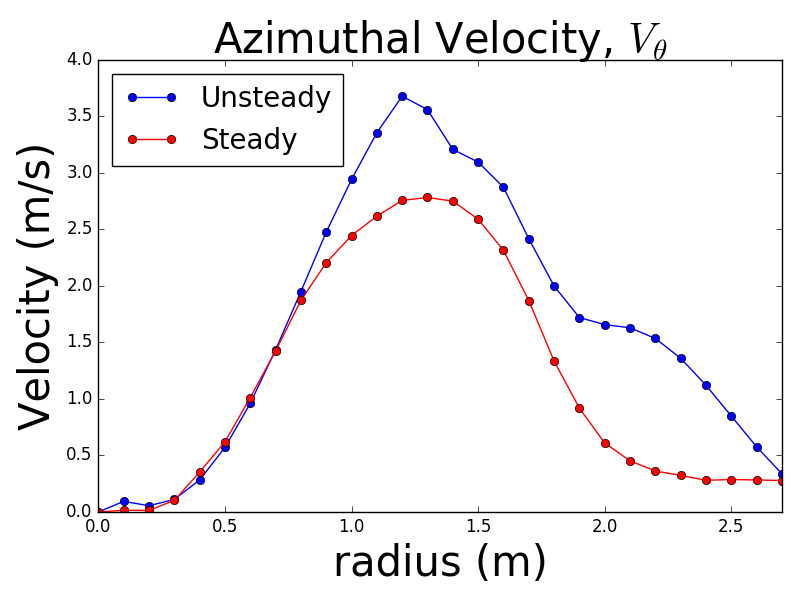
\includegraphics[width =0.7\textwidth]{figs/rom_radial}
 \caption{The azimuthal velocity profile as a function of radius for the
 steady and unsteady cases. The steady solution has a similar radial
 peak location, but a lower velocity magnitude and a more diffuse
 structure.}   
 \label{fig:rom_az}
\end{figure}


% The results between these simulations are broadly consistent. 
% Across a range of previously tested configurations the kinetic energy
% flux typically agrees to within 20\% and the sensitivities of the energy
% flux to small perturbations in the system configuration correlate well
% with the results of the higher fidelity transient model. 

\begin{figure}[htp!]
 \centering
 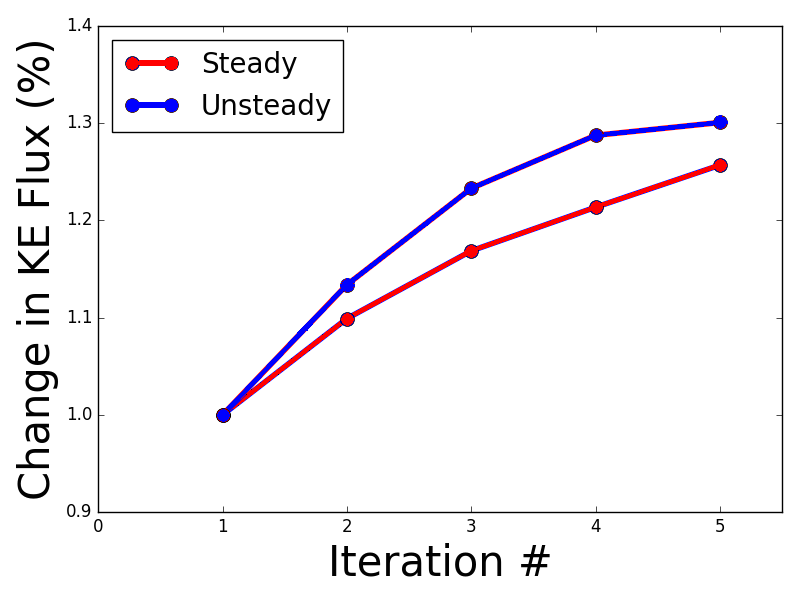
\includegraphics[width =0.7\textwidth]{figs/rom_iterate}
 \caption{A comparison between the change in kinetic energy flux due to
 a perturbation in system parameters between the steady and unsteady
 virtual vanes. For each iteration, a design parameter was changed, and
 the \% change in kinetic energy flux was recorded.}    
 \label{fig:rom_it}  
\end{figure}

\section{Field Configurations}
\label{sec:field_val}

Several field tests have been performed by the experimental team. After
each field test, qualitative observations, measurements and lessons
learned are provided by the field team. Actual measurements
are limited. Due to the complexity of the configuration
(two vane tiers and a cone) Gridded vanes cases have not been developed 
for the field. This section provides a discussion of some of
the results from the latest field test, as an example of typical
validations performed. 

 \begin{figure}[!htb]
  \begin{center}
   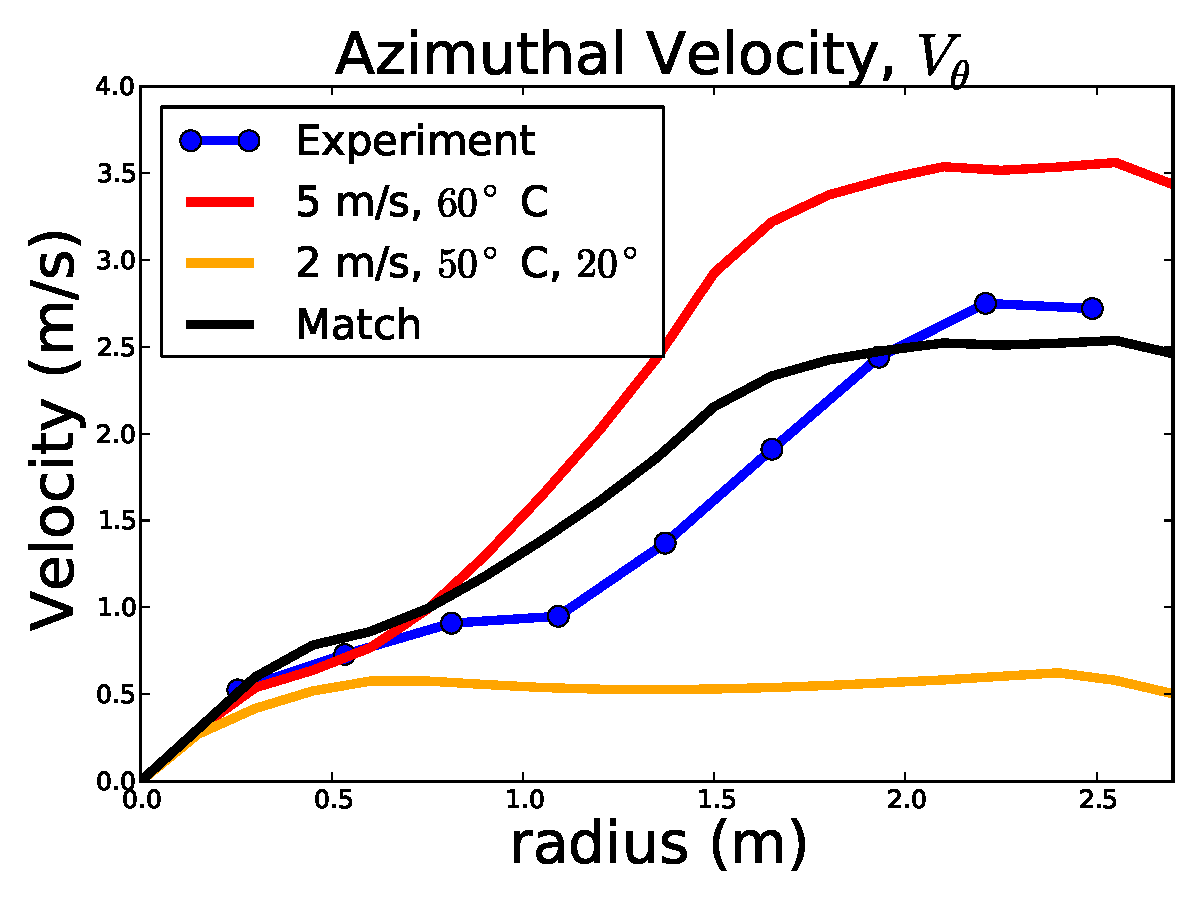
\includegraphics[width = 12 cm]{figs/validate_field}
   \caption{A comparison between simulated and experimental data for the
   August 2015 field test. Azimuthal velocity data from the actual field
   test is shown in blue. Two virtual vane simulations with different
   scenario parameters are shown in red and gold. The velocity field was
   temporally averaged but not averaged in space, to reproduce
   the measurements from the field.}
   \label{fig:field_val}
  \end{center}
 \end{figure}
%
% provide an example of these validations below
%

Figure~\ref{fig:field_val} shows data from the August 2015 field test in
blue. These results were obtained using an anonmometer at fixed
azimithal location (believed to be a ninety degree angle, where the zero
is defined to be aligned with the streamwise flow direction) to measure the
azimuthal velocity. The ultrasonic anemometer malfunctioned, and the
temperature was only measuered at one location at 1 meter height. A time
series from approximately an hour was gathered. This data included large
scenario uncertainties, with estimated 3 m/s variations in wind, 20
degree wind heading changes, and ten degree Celsius shifts in
temperature. A solidworks CAD file provided by the experimental team
defined the vane and cone geometry, which were then represented in the
simulations as virtual vanes and a solid surface, as described in 
Chapters~\ref{subsec:vane} and~\ref{subsec:solid_surface}. Hence, the
scenario uncertainly was significant, while the uncertainty in the
system apparatus was small. 

To span the range of scenario conditions, several simulations were conducted
with different parameters. These simulations were performed with
unsteady virtual vanes on a wind blown domain as detailed in
Section~\ref{sec:bc}.  
The azimuthal velocity from two such
simulations (red and gold lines) are plotted against the experimental
data (blue line) in Figure~\ref{fig:field_val}. The red line represents
an upper bound, with the strongest wind speeds and highest thermal
gradient. The gold line is a lower bound, with a more modest ambient
freestream velocity, a lower temperature gradient, and an indirect wind
heading. 

These simulations accurately bound the experimental data. Furthermore, a
``Matching'' case was identified that is broadly consistent with the
field results. This corresponded to a 3 m/s wind velocity and a 60
degree Celsius temperature gradient. 
As the rake was at fixed azimuthal location, the kinetic energy fluxes were
compared by assuming azimuthal symmetry and integrating in a horizontal
plane at the top of the vanes (where a turbine to extract this energy
would likely be placed). By this metric, the ``Matching'' simulation
kinetic energy flux agrees with the experimental estimate within
10\%. This is likely an optimistic measure, as the simulations indicate
that the velocity field is highly azimuthally asymmetric. Nevertheless,
no significant inconsistencies have been identified between the
experimental results and the simulations. 

%
% validation story is incomplete
% 
% you have done: 
%
% 1) comparions between laboratory + gridded + virtual 
% 
% 2) comparisons between gridded + virtual in laboratory
%    + field configurations, thermal only and wind
%
% 3) comparisons of virtual vanes to field observations 
%    quantitative + qualitative
%
%
% You need to discuss what needs to be validated -- the
% comparison to gridded vanes is a useful validation tool 
%
